\documentclass[12pt,twoside,a4paper]{report}
\usepackage[a4paper,width=150mm,top=25mm,bottom=25mm,bindingoffset=6mm]{geometry}

\usepackage[utf8x]{inputenc}
\usepackage[slovak]{babel}
\usepackage{palatino,verbatim}

% Balicek pre priamu rec - \say
\usepackage{dirtytalk}

% Balicek "alltt" je to iste ako "verbatim" mod, ale navyse podporuje aj formatovacie znacky textu
\usepackage{alltt}

% Obrazky
\usepackage{graphicx}
\graphicspath{ {obr/} }

% Cislovanie obrazkov a tabuliek
\usepackage{chngcntr}
%Cisluj obrazky nezavisle od cisla kapitol/podkapitol
\counterwithout{figure}{subsection}
\counterwithout{table}{subsection}

% Tabulky s viacriadkovymi bunkami a zlucenymi bunkami
% Tabulky generujem naastrojom "http://www.tablesgenerator.com/"
\usepackage{booktabs}
\usepackage{multirow}
% LaTeX ma problemy s prikazmi cline a cmidrule, ked je babel nastaveny na slovencinu/cestinu, kvoli definicii pomlcky
\usepackage{etoolbox}
\preto\tabular{\shorthandoff{-}}

%Uloz obrazok tam, kde je deklarovany
%\usepackage[subsection]{placeins}

\newcommand\sktxt[1]{\foreignlanguage{slovak}{#1}}

\begin{document}
\pagenumbering{arabic}

\setcounter{chapter}{1}
\chapter*{Multi-area OSPF}
\paragraph{}
Andrej Šišila, Marián Vachalík

\tableofcontents

\newpage
\section{Topológia}
\paragraph{}
Budeme konfigurovať Multi-area OSPF, ktorá je znázornená na obrázku \ref{fig:multiarea_ospf_topo}. Smerovač R10 patrí tiež do oblasti 4. IP adresácia je uvedená v tabuľke \ref{tab:ip_adresacia} a dopĺňa grafické znázornenie topológie na obrázku \ref{fig:multiarea_ospf_topo}.

\begin{figure}[!htb]
\centering
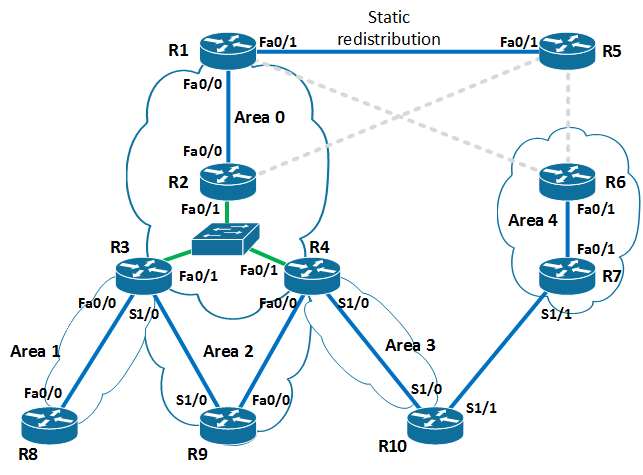
\includegraphics[width=12cm,keepaspectratio]{multiarea_ospf_topo}
\caption{Topológia Multi-area OSPF}
\label{fig:multiarea_ospf_topo}
\end{figure}



\begin{table}[!htb]
\centering
\caption{IP adresácia}
\label{tab:ip_adresacia}
\begin{tabular}{|c|c|l|l|l|}
\hline
\multicolumn{1}{|c|}{\textbf{Smerovač}}    & \multicolumn{1}{c|}{\textbf{Funkcia}}                        & \multicolumn{1}{c|}{\textbf{Rozhranie}} & \multicolumn{1}{c|}{\textbf{IP adresa}} & \multicolumn{1}{c|}{\textbf{Maska}} \\ \hline
\multirow{3}{*}{R1}  & \multirow{3}{*}{ASBR}                   & Fa0/0                                   & 10.0.12.1                               & 255.255.255.0                       \\ \cline{3-5} 
                     &                                         & Fa0/1                                   & 10.100.15.1                             & 255.255.255.0                       \\ \cline{3-5} 
                     &                                         & Lo0                                     & 10.255.255.1                            & 255.255.255.255                     \\ \hline
\multirow{3}{*}{R2}  & \multirow{3}{*}{Štandardný}             & Fa0/0                                   & 10.0.12.2                               & 255.255.255.0                       \\ \cline{3-5} 
                     &                                         & Fa0/1                                   & 10.0.234.2                             & 255.255.255.0                       \\ \cline{3-5} 
                     &                                         & Lo0                                     & 10.255.255.2                            & 255.255.255.255                     \\ \hline
\multirow{4}{*}{R3}  & \multirow{4}{*}{ABR}                    & Fa0/0                                   & 10.1.38.1                               & 255.255.255.0                       \\ \cline{3-5} 
                     &                                         & Fa0/1                                   & 10.0.234.3                              & 255.255.255.0                       \\ \cline{3-5} 
                     &                                         & S1/0                                    & 10.2.39.1                               & 255.255.255.252                     \\ \cline{3-5} 
                     &                                         & Lo0                                     & 10.255.255.3                            & 255.255.255.255                     \\ \hline
\multirow{4}{*}{R4}  & \multirow{4}{*}{ABR}                    & Fa0/0                                   & 10.2.49.1                               & 255.255.255.0                       \\ \cline{3-5} 
                     &                                         & Fa0/1                                   & 10.0.234.4                              & 255.255.255.0                       \\ \cline{3-5} 
                     &                                         & S1/0                                    & 10.3.104.1                              & 255.255.255.252                     \\ \cline{3-5} 
                     &                                         & Lo0                                     & 10.255.255.4                            & 255.255.255.255                     \\ \hline
\multirow{2}{*}{R5}  & \multirow{2}{*}{Smerovač iného systému} & Fa0/1                                   & 10.100.15.2                             & 255.255.255.0                       \\ \cline{3-5} 
                     &                                         & Lo0                                     & 10.255.255.5                            & 255.255.255.255                     \\ \hline
\multirow{2}{*}{R6}  & \multirow{2}{*}{Štandardný}             & Fa0/0                                   & 10.4.67.1                               & 255.255.255.0                       \\ \cline{3-5} 
                     &                                         & Lo0                                     & 10.255.255.6                            & 255.255.255.255                     \\ \hline
\multirow{3}{*}{R7}  & \multirow{3}{*}{Štandardný}             & Fa0/1                                   & 10.4.67.2                               & 255.255.255.0                       \\ \cline{3-5} 
                     &                                         & S1/1                                    & 10.4.107.1                              & 255.255.255.0                       \\ \cline{3-5} 
                     &                                         & Lo0                                     & 10.255.255.7                            & 255.255.255.255                     \\ \hline
\multirow{2}{*}{R8}  & \multirow{2}{*}{Štandardný}             & Fa0/0                                   & 10.1.38.2                               & 255.255.255.0                       \\ \cline{3-5} 
                     &                                         & Lo0                                     & 10.255.255.8                            & 255.255.255.255                     \\ \hline
\multirow{3}{*}{R9}  & \multirow{3}{*}{Štandardný}             & Fa0/0                                   & 10.2.49.2                               & 255.255.255.0                       \\ \cline{3-5} 
                     &                                         & S1/0                                    & 10.2.39.2                               & 255.255.255.0                       \\ \cline{3-5} 
                     &                                         & Lo0                                     & 10.255.255.9                            & 255.255.255.255                     \\ \hline
\multirow{3}{*}{R10} & \multirow{3}{*}{ABR}                    & S1/0                                    & 10.3.104.2                              & 255.255.255.0                       \\ \cline{3-5} 
                     &                                         & S1/1                                    & 10.4.107.2                              & 255.255.255.0                       \\ \cline{3-5} 
                     &                                         & Lo0                                     & 10.255.255.10                           & 255.255.255.255                     \\ \hline
\end{tabular}
\end{table}


% Novu kapitolu davam na novu stranu, lebo bez toho mi zobrazuje tabulku v dalsej kapitole, kde ale tabulka nepatri.
\newpage


\section{Úlohy a ich konfigurácia}
\subsection{Základná konfigurácia}
\subsubsection{Popis}
\paragraph{}
Ako za základnú konfiguráciu považujeme nastavenie adresácie, vzdialeného prístupu a vypisovania konzoly. IP adresy sme vytvárali tak, že prvý oktet bola 10, druhý oktet bolo číslo oblasti, tretí oktet bolo číslo, ktoré vzniklo ako spojenie čísel dvojíc smerovačov, medzi ktorými sa sieť nachádzala; napr. sieť medzi smerovačmi 4 a 10 by bol tretí oktet 104, medzi smerovačmi R1 a R2 by to bolo 12 atď. Každý smerovač má aj svoje loopback rozhranie, ktoré bližšie opisujeme v kapitole \say{Router-id - loopback0, passive-interface}.

\subsubsection{Konfigurácia}
\noindent
{\fontfamily{qcr}\selectfont
\begin{small}
\begin{verbatim}
!!!!!!!!!!   R1   !!!!!!!!!!
hostname R1
no ip domain-lookup
username admin privilege 15 secret admin
line con 0
	login local
	logging synchronous
	exec-timeout 120
line vty 0 15
	privilege level 15
	no login
int lo1
	ip address 10.255.255.1 255.255.255.255
	no shutdown
int f0/1
	ip address 10.100.15.1 255.255.255.0
	no shutdown
int f0/0
	ip address 10.0.12.1 255.255.255.0
	no shutdown

do show ip interface brief


!!!!!!!!!!   R2   !!!!!!!!!!
hostname R2
no ip domain-lookup
username admin privilege 15 secret admin
line con 0
	login local
	logging synchronous
	! Predĺženie intervalu na odpojenie používateľa od konzoly
	exec-timeout 120
line vty 0 15
	privilege level 15
	no login
int lo1
	ip address 10.255.255.2 255.255.255.255
	no shutdown
int f0/1
	ip address 10.0.234.2 255.255.255.0
	no shutdown
int f0/0
	ip address 10.0.12.2 255.255.255.0
	no shutdown

do show ip interface brief


!!!!!!!!!!   R3   !!!!!!!!!!
hostname R3
no ip domain-lookup
username admin privilege 15 secret admin
line con 0
	login local
	logging synchronous
	exec-timeout 120
line vty 0 15
	privilege level 15
	no login
int lo1
	ip address 10.255.255.3 255.255.255.255
	no shutdown
int f0/1
	ip address 10.0.234.3 255.255.255.0
	no shutdown
int f0/0
	ip address 10.1.38.1 255.255.255.0
	no shutdown
int s1/0
	ip address 10.2.39.1 255.255.255.252
	no shutdown

do show ip interface brief


!!!!!!!!!!   R4   !!!!!!!!!!
hostname R4
no ip domain-lookup
username admin privilege 15 secret admin
line con 0
	login local
	logging synchronous
	exec-timeout 120
line vty 0 15
	privilege level 15
	no login
int lo1
	ip address 10.255.255.4 255.255.255.255
	no shutdown
int f0/1
	ip address 10.0.234.4 255.255.255.0
	no shutdown
int f0/0
	ip address 10.2.49.1 255.255.255.0
	no shutdown
int s1/0
	ip address 10.3.104.1 255.255.255.252
	no shutdown

do show ip interface brief


!!!!!!!!!!   R5   !!!!!!!!!!
hostname R5
no ip domain-lookup
username admin privilege 15 secret admin
line con 0
	login local
	logging synchronous
	exec-timeout 120
line vty 0 15
	privilege level 15
	no login
int lo1
	ip address 10.255.255.5 255.255.255.255
	no shutdown
int f0/1
	ip address 10.100.15.2 255.255.255.0
	no shutdown

do show ip interface brief

!!!!!!!!!!   R6   !!!!!!!!!!
hostname R6
no ip domain lookup
username admin privil 15 secret admin
line con 0
	login local
	logging synchro
	exec-timeout 120
line vty 0 15
	privilege level 15	
	no login
int lo1
	ip add 10.255.255.6 255.255.255.255
	no sh
int fa0/1 
	ip add 10.4.67.1 255.255.255.0
	no sh

!!!!!!!!!!   R7   !!!!!!!!!!
hostname R7
no ip domain lookup
username admin privil 15 secret admin
line con 0
	login local
	logging synchro
	exec-timeout 120
line vty 0 15
	privilege level 15	
	no login
int lo1
	ip add 10.255.255.7 255.255.255.255
	no sh
int fa0/1 
	ip add 10.4.67.2 255.255.255.0
	no sh
int s1/1
	ip add 10.4.107.1 255.255.255.0
	no sh

!!!!!!!!!!   R8   !!!!!!!!!!
hostname R8
no ip domain lookup
username admin privil 15 secret admin
line con 0
	login local
	logging synchro
	exec-timeout 120
line vty 0 15
	privilege level 15	
	no login
int lo1
	ip add 10.255.255.8 255.255.255.255
	no sh
int fa0/0 
	ip add 10.1.38.2 255.255.255.0
	no sh

!!!!!!!!!!   R9   !!!!!!!!!!
hostname R9
no ip domain lookup
username admin privil 15 secret admin
line con 0
	login local
	logging synchro
	exec-timeout 120
line vty 0 15
	privilege level 15	
	no login
int lo1
	ip add 10.255.255.9 255.255.255.255
	no sh
int fa0/0 
	ip add 10.2.49.2 255.255.255.0
	no sh
int s1/0
	ip add 10.2.39.2 255.255.255.0
	no sh

!!!!!!!!!!   R10   !!!!!!!!!!
hostname R10
no ip domain lookup
username admin privil 15 secret admin
line con 0
	login local
	logging synchro
	exec-timeout 120
line vty 0 15
	privilege level 15	
	no login
int lo1
	ip add 10.255.255.10 255.255.255.255
	no sh
int s1/1 
	ip add 10.4.107.2 255.255.255.0
	no sh
int s1/0
	ip add 10.3.104.2 255.255.255.0
	no sh
\end{verbatim}
\end{small}
}

\subsubsection{Overenie}
\paragraph{}
Základnú konfiguráciu sme overili príkazmi \say{show ip interface brief}, \say{show cdp neighbors}. Nižšie sú uvedené výpisy zo smerovača R3.

\noindent
{\fontfamily{qcr}\selectfont
\begin{small}
\begin{verbatim}

R3#show ip interface brief 
Interface                  IP-Address      OK? Method Status   Protocol
FastEthernet0/0            10.1.38.1       YES TFTP   up       up      
FastEthernet0/1            10.0.234.3      YES TFTP   up       up      
Serial1/0                  10.2.39.1       YES TFTP   up       up      
Serial1/1                  unassigned      YES TFTP   up       down    
Serial1/2                  unassigned      YES TFTP   up       down    
Serial1/3                  unassigned      YES TFTP   up       down    
Loopback1                  10.255.255.3    YES TFTP   up       up      


R3#show cdp neighbors 
Capability Codes: R - Router, T - Trans Bridge, B - Source Route Bridge
                  S - Switch, H - Host, I - IGMP, r - Repeater

Device ID        Local Intrfce     Holdtme    Capability  Platform  Port ID
R2               Fas 0/1            125         R S I     2691      Fas 0/1
R4               Fas 0/1            137         R S I     2691      Fas 0/1
R8               Fas 0/0            155         R S I     2691      Fas 0/0
R9               Ser 1/0            147         R S I     2691      Ser 1/0

\end{verbatim}
\end{small}
}

\paragraph{}
Z výpisov vyplýva, že smerovač R3 susedí so štyrmi ďalšími smerovačmi: R2, R4, R8 a R9. Má vlastný aktívny loopback (viď kapitolu \say{Router-id - loopback0, passive-interface}). R3 na rozhraní \say{Fas 0/1} susedí s dvoma smerovačmi R2 a R4, pretože sú pripojené ku prepínaču, čím R2, R3 a R4 tvoria broadcastovú doménu.

\subsection{Nakonfigurovať OSPF s viacerými oblasťami}
\subsubsection{Popis}
\paragraph{}
Jednotlivé smerovače sme priradili do oblastí podľa obrázku \ref{fig:multiarea_ospf_topo}.

\subsubsection{Konfigurácia}
\noindent
{\fontfamily{qcr}\selectfont

% Urob text mensi, aby sa vosiel na sirku obrazovky
\begin{small}

% Pouzijeme "verbatim", aby sme escapeovali cely odsek
\begin{verbatim}
!KONFIGURACIA R1
router ospf 1
    network 10.255.255.1 0.0.0.0 area 0
    exit
int f0/0
    ip ospf 1 area 0
    !treba zapnut interface, ked nam padne router/server
    no shutdown

!KONFIGURACIA R2
router ospf 1
    network 10.255.255.2 0.0.0.0 area 0
    exit
int f0/0
    ip ospf 1 area 0
    no shutdown
int f0/1
    ip ospf 1 area 0
    no shutdown

!KONFIGURACIA R3
router ospf 1
    network 10.255.255.3 0.0.0.0 area 1
    exit
int f0/1
    ip ospf 1 area 0
    no shutdown
int f0/0
    ip ospf 1 area 1
    no shutdown
int s1/0
    ip ospf 1 area 2
    no shutdown

!KONFIGURACIA R4
router ospf 1
    network 10.255.255.4 0.0.0.0 area 3
    exit
int f0/1
    ip ospf 1 area 0
    no shutdown
int f0/0
    ip ospf 1 area 2
    no shutdown
int s1/0
    ip ospf 1 area 3
    no shutdown


!KONFIGURACIA R5
ip route 0.0.0.0 0.0.0.0 f0/1 10.100.15.1

!KONFIGURACIA R6
router ospf 1
    network 10.255.255.6 0.0.0.0 area 4
    exit
int f0/1
    ip ospf 1 area 4
    no sh

!KONFIGURACIA R7
router ospf 1
    network 10.255.255.7 0.0.0.0 area 4
    exit
int f0/1
    ip ospf 1 area 4
    no sh
int s1/1
    ip ospf 1 area 4
    no sh

!KONFIGURACIA R8
router ospf 1
    network 10.255.255.8 0.0.0.0 area 1
    exit
int f0/0
    ip ospf 1 area 1
    no sh

!KONFIGURACIA R9
router ospf 1
    network 10.255.255.9 0.0.0.0 area 2
    exit
int f0/0
    ip ospf 1 area 2
    no sh
int s1/0
    ip ospf 1 area 2
    no sh 

!KONFIGURACIA R10
router ospf 1
    network 10.255.255.10 0.0.0.0 area 3
    exit
int s1/0
    ip ospf 1 area 3
    no sh
int s1/1
    ip ospf 1 area 4
    no sh
\end{verbatim}
\end{small}
}

\subsubsection{Overenie}
\paragraph{}
Príslušnosť smerovačov do oblastí sme testovali týmito príkazmi \say{show ip ospf interface brief}, \say{show ip ospf neighbors}, \say{show ip ospf database}. Nižšie uvádzame výpis uvedených príkazov zo smerovača R1.

\noindent
{\fontfamily{qcr}\selectfont
\begin{small}
\begin{alltt}

R1#show ip ospf interface f0/0
FastEthernet0/0 is up, line protocol is up 
  \textbf{Internet Address 10.0.12.1/24, Area 0}
  ...

\end{alltt}
\end{small}
}

\noindent
{\fontfamily{qcr}\selectfont
\begin{small}
\begin{verbatim}
R1#show ip ospf database 

            OSPF Router with ID (10.255.255.1) (Process ID 1)

		Router Link States (Area 0)

Link ID         ADV Router      Age         Seq#       Checksum Link count
10.255.255.1    10.255.255.1    748         0x800000A8 0x00D192 4
10.255.255.2    10.255.255.2    835         0x800000A7 0x0046AC 4
10.255.255.3    10.255.255.3    707         0x800000A4 0x00D1B1 1
10.255.255.4    10.255.255.4    811         0x800000A5 0x00CFCA 2
10.255.255.10   10.255.255.10   3     (DNA) 0x80000002 0x006AD7 1

		Net Link States (Area 0)

Link ID         ADV Router      Age         Seq#       Checksum
10.0.234.4      10.255.255.4    811         0x800000A4 0x00F073

		Summary Net Link States (Area 0)

Link ID         ADV Router      Age         Seq#       Checksum
10.1.38.0       10.255.255.3    707         0x800000A3 0x000A48
10.2.39.0       10.255.255.3    707         0x8000009F 0x009B42
10.2.39.0       10.255.255.4    811         0x8000009F 0x00110C
10.2.39.3       10.255.255.3    707         0x8000009F 0x00E835
10.2.39.3       10.255.255.4    813         0x8000009F 0x006379
10.2.49.0       10.255.255.3    709         0x8000009F 0x000FFA
10.2.49.0       10.255.255.4    813         0x8000009F 0x002231
10.3.104.0      10.255.255.4    813         0x8000009F 0x00BBDE
10.3.104.0      10.255.255.10   7     (DNA) 0x80000001 0x005221
10.3.104.3      10.255.255.4    813         0x8000009F 0x0009D1
10.3.104.3      10.255.255.10   7     (DNA) 0x80000001 0x00A48E
10.4.67.0       10.255.255.10   7     (DNA) 0x80000001 0x00434A
10.4.107.0      10.255.255.10   7     (DNA) 0x80000001 0x00254A
10.255.255.3    10.255.255.3    709         0x800000A3 0x00413E
10.255.255.4    10.255.255.4    813         0x800000A3 0x00314C
10.255.255.4    10.255.255.10   7     (DNA) 0x80000001 0x00D405
10.255.255.6    10.255.255.10   7     (DNA) 0x80000001 0x0025A8
10.255.255.7    10.255.255.10   7     (DNA) 0x80000001 0x00B620
10.255.255.8    10.255.255.3    709         0x80000021 0x00787A
10.255.255.9    10.255.255.3    710         0x8000009F 0x008FAD
10.255.255.9    10.255.255.4    814         0x8000009F 0x000577
10.255.255.10   10.255.255.4    814         0x8000009F 0x007FBB
10.255.255.10   10.255.255.10   7     (DNA) 0x80000001 0x0016FD

		Router Link States (Area 3)

Link ID         ADV Router      Age         Seq#       Checksum Link count
10.255.255.1    10.255.255.1    245         0x800000A4 0x006F18 0

		Type-5 AS External Link States

Link ID         ADV Router      Age         Seq#       Checksum Tag
10.255.255.5    10.255.255.1    1515        0x8000009E 0x009ACE 0

\end{verbatim}
\end{small}
}

\paragraph{}
Z výpisu \say{show ip ospf interface f0/0} smerovača R1 vyplýva, že rozhranie \say{f0/0} patrí do oblasti 0, čo je chrbticová oblasť. V OSPF topológií majú smerovače v rovnakej oblasti totožnú LSDB (Link State databázu). Na začiatku výpisu LSDB vidíme \say{Router ID} smerovača, ktorého databázu sledujeme. V časti \say{Router Link States (Area 0)} vidíme priamo pripojené siete ku chrbticovej oblasti. Šíria sa ako LSA 1 a generuje ich každý smerovač v OSPF topológií. Je medzi nimi aj loopback rozhranie R10, pretože sme museli vytvoriť virtuálne pripojenie oblasti 4 cez oblasť 3 (viď kapitola \say{Area 3 – Stub}). R10 sa preto tvári ako ABR a šíri svoje siete správami LSA 3. V časti \say{Net Link States (Area 0)} vidíme DR smerovač (R4). Šíria sa ako LSA 2 a generuje ich DR smerovač. V časti \say{Summary Net Link States (Area 0)} vidíme ohlasované siete od ABR smerovačov. Niektoré záznamy sú zdvojené, pretože aj R3, aj R4 sú ABR smerovačmi do oblasti 2. Šíria sa ako LSA 3 a generujú ich ABR smerovače. V časti \say{Type-5 AS External Link States} vidíme siete ohlasované z iných autonómnych systémov (AS). V našom prípade sme ohlasovali cestu ku smerovaču R5. R5 bol pripojený ku R1, preto sa stal R1 ASBR smerovačom. Tieto siete sa šíria ako LSA 5 a generuje ich ASBR smerovač.



\subsection{R2, R3, R4 broadcast spojenia prostredníctvom L2 prepínača, zvyšok spojení P2P}
\subsubsection{Popis}
\paragraph{}
V \say{broadcastovej} a \say{non-broadcastovej} doméne smerovače v rámci OSPF topológie komunikujú pomocou LSA 2 správ, ktorými si volia DR/BDR smerovač. DR (Designated Router) je smerovač, ktorý slúži ako centrálny bod pre výmenu smerovacích informácií v \say{broadcast} doméne v rámci OSPF. BDR (Backup DR) je záložný smerovač v prípade, že by DR smerovač prestal fungovať.

\subsubsection{Konfigurácia}

\noindent
{\fontfamily{qcr}\selectfont

% Urob text mensi, aby sa vosiel na sirku obrazovky
\begin{small}

% Pouzijeme "verbatim", aby sme escapeovali cely odsek
\begin{verbatim}
!KONFIGURACIA R1
int f0/0
    ip ospf network point-to-point

!KONFIGURACIA R2
int f0/0
    ip ospf network point-to-point

!KONFIGURACIA R3
int f0/0
    ip ospf network point-to-point
int s1/0
    ip ospf network point-to-point

!KONFIGURACIA R4
int f0/0
    ip ospf network point-to-point
int s1/0
    ip ospf network point-to-point

!KONFIGURACIA R6
int f0/1
    ip ospf network point-to-point

!KONFIGURACIA R7
int f0/1
    ip ospf network point-to-point
int s1/1
    ip ospf network point-to-point

!KONFIGURACIA R8
int f0/0
    ip ospf network point-to-point

!KONFIGURACIA R9
int f0/0
    ip ospf network point-to-point
    ip ospf 1 area 2
int s1/0
    ip ospf network point-to-point

!KONFIGURACIA R10
int s1/0
    ip ospf network point-to-point
int s1/1
    ip ospf network point-to-point
\end{verbatim}

\end{small}

}

\subsubsection{Overenie}
\paragraph{}
Typ siete (resp. rozhrania) sme overovali príkazom \say{show ip ospf interface \textless názov\_rozhrania \textgreater }. Napríklad smerovač R3 na Fa0/0:

\noindent
{\fontfamily{qcr}\selectfont
\begin{small}
\begin{alltt}
FastEthernet0/0 is up, line protocol is up 
  Internet Address 10.1.38.1/24, Area 1 
  Process ID 1, Router ID 10.255.255.3, \textbf{Network Type POINT_TO_POINT}, Cost: 10
\end{alltt}
\end{small}
}

\paragraph{}
Z uvedeného show príkazu vyplýva, že rozhranie \say{Fa0/0} na smerovači R3 patrí do siete typu \say{point-to-point}.

\subsection{Router–id – loopback0, passive–interface}
\subsubsection{Popis}
\paragraph{}
IP adresa loopback rozhrania sa nastavila ako Router ID a zároveň sme loopback rozhranie \say{lo1} nastavili ako pasívne.

\subsubsection{Konfigurácia}
\paragraph{}
Na každom routri sme vykonali tieto príkazy:
\noindent
{\fontfamily{qcr}\selectfont

% Urob text mensi, aby sa vosiel na sirku obrazovky
\begin{small}

% Pouzijeme "verbatim", aby sme escapeovali cely odsek
\begin{verbatim}
router ospf 1
    router-id 10.255.255.X
    passive-interface lo1
\end{verbatim}
\end{small}
}


'X' symbolizuje číslo smerovača (napr. pre R1: 10.255.255.1)

\subsubsection{Overenie}
\paragraph{}
Router ID sme overovali príkazom \say{show ip ospf 1}.

\noindent
{\fontfamily{qcr}\selectfont
\begin{small}
\begin{verbatim}
R3#show ip ospf 1
 Routing Process "ospf 1" with ID 10.255.255.3
\end{verbatim}
\end{small}
}

\paragraph{}
Pasívne rozhranie sme overovali príkazom \say{show ip ospf interface brief}.

\noindent
{\fontfamily{qcr}\selectfont
\begin{small}
\begin{alltt}

R3#show ip ospf interface brief
Interface    PID   Area            IP Address/Mask    Cost  State Nbrs F/C
Fa0/1        1     0               10.0.234.3/24      1     DR    2/2
\textbf{Lo1          1     1               10.255.255.3/32    1     LOOP  0/0}
Fa0/0        1     1               10.1.38.1/24       10    P2P   1/1
Se1/0        1     2               10.2.39.1/30       64    P2P   1/1

\end{alltt}
\end{small}
}

\paragraph{}
Z výpisu vyplýva, že loopback rozhranie \say{Lo1} je v pasívnom móde (LOOP) a teda sa cezeň nemôže vytvoriť susedstvo.

\subsection{Area 1 – Totally Stubby}
\subsubsection{Popis}
\paragraph{}
\say{Totally Stuby} oblasť je taký druh oblasti, v ktorej sa nešíria žiadne LSA 3, LSA 4, LSA 5 a predvolená cesta sa šíri ako LSA 3.

\subsubsection{Konfigurácia}
\paragraph{}
Oblasť 1 nastavíme na typ \say{Tottaly Stuby} na smerovačoch R3 a R8.

\noindent
{\fontfamily{qcr}\selectfont
\begin{small}
\begin{verbatim}

!R3 - R3 je ABR, preto použijeme dodatočný príkaz "no-summary", aby sme 
!definovali Totally Stuby oblasť
R3(config)#router ospf 1
R3(config-router)#area 1 stub no-summary

\end{verbatim}
\end{small}
}

\noindent
{\fontfamily{qcr}\selectfont
\begin{small}
\begin{verbatim}

!R8
R8(config)#router ospf 1
R8(config-router)#area 1 stub

\end{verbatim}
\end{small}
}

\subsubsection{Overenie}
\paragraph{}
Na overenie sme použili príkaz \say{show ip ospf database}. 

\noindent
{\fontfamily{qcr}\selectfont
\begin{small}
\begin{verbatim}

R3#show ip ospf database

...

                Router Link States (Area 1)

Link ID         ADV Router      Age         Seq#       Checksum Link count
10.255.255.3    10.255.255.3    23          0x80000088 0x008854 3
10.255.255.8    10.255.255.8    24          0x80000081 0x0021B8 3

		Summary Net Link States (Area 1)

Link ID         ADV Router      Age         Seq#       Checksum
0.0.0.0         10.255.255.3    68          0x80000001 0x0045EB

...

\end{verbatim}
\end{small}
}

\paragraph{}
Z príkazu \say{show ip ospf database} na R3 vyplýva, že predvolená cesta sa v oblasti 1 šíri ako predvolená cesta ako LSA 3 (Link ID t.j. Router ID v časti \say{Summary Net Link States} pre oblasť 1 je 0.0.0.0).

\subsection{Area 3 – Stub}
\subsubsection{Popis}
\paragraph{}
Oblasť 3 nemôže byť \say{Stub} oblasťou, pretože sa ňou nešíria správy LSA 4 a 5, ktoré potrebuje virtuálne spojenie. Preto sme po úvahe oblasť 3 zmenili zo \say{Stub} na štandardnú oblasť a namiesto toho sme oblasť 2 nastavili ako \say{Stub}.

\subsubsection{Konfigurácia}
\paragraph{}
Konfigurovali sme smerovače R3, R4 a R9. Konfigurácia bola zhodná pre všetky spomenuté smerovače.

\noindent
{\fontfamily{qcr}\selectfont
\begin{small}
\begin{verbatim}

R3(config)#router ospf 1
R3(config-router)#area 2 stub

\end{verbatim}
\end{small}
}

\subsubsection{Overenie}
\paragraph{}
Stub sieť sme overili príkazom \say{show ip ospf database router} zo smerovača R3 a R4.


\noindent
{\fontfamily{qcr}\selectfont
\begin{small}
\begin{alltt}
R3#show ip ospf database router
...
		Router Link States (Area 2)
...

  LS age: 2012
  Options: (No TOS-capability, DC)
  LS Type: Router Links
  \textbf{Link State ID: 10.255.255.3}
  Advertising Router: 10.255.255.3
  LS Seq Number: 80000008
  Checksum: 0x2FDB
  Length: 48
  Area Border Router
  Number of Links: 2

    Link connected to: another Router (point-to-point)
     (Link ID) Neighboring Router ID: 10.255.255.9
     (Link Data) Router Interface address: 10.2.39.1
      Number of TOS metrics: 0
       TOS 0 Metrics: 64

    \textbf{Link connected to: a Stub Network}
     (Link ID) Network/subnet number: 10.2.39.0
     (Link Data) Network Mask: 255.255.255.252
      Number of TOS metrics: 0
       TOS 0 Metrics: 64

...

\end{alltt}
\end{small}
}


\noindent
{\fontfamily{qcr}\selectfont
\begin{small}
\begin{alltt}
R4#show ip ospf database router
...
		Router Link States (Area 2)
...

          
  LS age: 510
  Options: (No TOS-capability, DC)
  LS Type: Router Links
  \textbf{Link State ID: 10.255.255.4}
  Advertising Router: 10.255.255.4
  LS Seq Number: 80000008
  Checksum: 0xB6BB
  Length: 48
  Area Border Router
  Number of Links: 2

    Link connected to: another Router (point-to-point)
     (Link ID) Neighboring Router ID: 10.255.255.9
     (Link Data) Router Interface address: 10.2.49.1
      Number of TOS metrics: 0
       TOS 0 Metrics: 65535

    \textbf{Link connected to: a Stub Network}
     (Link ID) Network/subnet number: 10.2.49.0
     (Link Data) Network Mask: 255.255.255.0
      Number of TOS metrics: 0
       TOS 0 Metrics: 65535
...

\end{alltt}
\end{small}
}

\paragraph{}
Z uvedeých výpisov vyplýva, že smerovače R3 a R4 patria k oblasti 2, čo je oblasť typu \say{Stub}.

\subsection{Area 4 – pripojenie pomocou virtuálnej linky}
\subsubsection{Popis}
\paragraph{}
Oblasť 4 sme potrebovali pripojiť ku existujúcej OSPF topológií. Pripojenie sa dalo uskutočniť iba cez oblasť 3, čo nie je chrbticová oblasť. Keďže každá oblasť v OSPF topológií musí byť pripojená ku chrbticovej oblasti. Preto sme museli oblasť 4 pripojiť ku chrbticovej oblasti tak, že sme vytvorili vzájomné virtuálne spojenie medzi smerovačmi R4 a R10.

\subsubsection{Konfigurácia}
\paragraph{}
Nižšie je uvedená konfigurácia smerovačov R4 a R10.

\noindent
{\fontfamily{qcr}\selectfont
\begin{small}
\begin{verbatim}
!R4
router ospf 1
    area 3 virtual-link 10.255.255.10

\end{verbatim}
\end{small}
}

\noindent
{\fontfamily{qcr}\selectfont
\begin{small}
\begin{verbatim}
!R10
router ospf 1
    area 3 virtual-link 10.255.255.4

\end{verbatim}
\end{small}
}

\subsubsection{Overenie}
\paragraph{}
Virtuálne pripojenie sme overovali príkazom \say{show ip ospf interface brief} na smerovačoch R4 a R10 a príkazom \say{show ip ospf database} na R4 (pretože pokiaľ virtuálne pripojenie funguje, záznamy o sieťach v oblasti 4 by mali byť vidieť v chrbticovej oblasti).

\noindent
{\fontfamily{qcr}\selectfont
\begin{small}
\begin{alltt}
R4#show ip ospf interface brief 
Interface    PID   Area            IP Address/Mask    Cost  State Nbrs F/C
\textbf{VL0          1     0               10.3.104.1/30      64    P2P   1/1}
Fa0/1        1     0               10.0.234.4/24      10    DROTH 2/2
Fa0/0        1     2               10.2.49.1/24       65535 P2P   1/1
Lo1          1     3               10.255.255.4/32    1     LOOP  0/0
Se1/0        1     3               10.3.104.1/30      64    P2P   1/1


R10#show ip ospf interface brief 
Interface    PID   Area            IP Address/Mask    Cost  State Nbrs F/C
\textbf{VL0          1     0               10.3.104.2/24      64    P2P   1/1}
Lo1          1     3               10.255.255.10/32   1     LOOP  0/0
Se1/0        1     3               10.3.104.2/24      64    P2P   1/1
Se1/1        1     4               10.4.107.2/24      64    P2P   1/1



R4#show ip ospf database 
...
		Summary Net Link States (Area 0)

Link ID         ADV Router      Age         Seq#       Checksum
...
10.4.67.0       10.255.255.10   5     (DNA) 0x80000001 0x00434A
10.4.107.0      10.255.255.10   5     (DNA) 0x80000001 0x00254A
...
10.255.255.6    10.255.255.10   5     (DNA) 0x80000001 0x0025A8
10.255.255.7    10.255.255.10   5     (DNA) 0x80000001 0x00B620
...
\end{alltt}
\end{small}
}

\paragraph{}
Z výpisov od oboch smerovačov vyplýva, že virtuálne pripojenie bolo úspešne vytvorené a malo názov \say{VL0}. Záznamy sietí z oblasti 4 sú vidieť v LSDB databáze na R4 šírené ako LSA 3, čo znamená, že sa oblasť 4 tvári ako priamo pripojená ku chrbticovej oblasti.

\subsection{Statická redistribúcia smerovacích záznamov z R5}
\subsubsection{Popis}
\paragraph{}
Na smerovači R5 sme nastavili predvolenú cestu, aby sme prepojili smerovač externej oblasti, R5, s OSPF topológiou.

\subsubsection{Konfigurácia}
\noindent
{\fontfamily{qcr}\selectfont
\begin{small}
\begin{verbatim}

R5(config)#ip route 0.0.0.0 0.0.0.0 f0/1 10.100.15.1

\end{verbatim}
\end{small}
}

\paragraph{}
Potom sme na smerovači R1 namapovali cestu k "lo1" na R5, ktorú sme ohlásili v rámci OSPF topológie príkazmi "redistribute":

\noindent
{\fontfamily{qcr}\selectfont
\begin{small}
\begin{verbatim}

R1(config)#ip route 10.255.255.5 255.255.255.255 f0/1 10.100.15.2
R1(config)#router ospf 1
R1(config-router)#redistribute static subnets
R1(config-router)#redistribute connected subnets

\end{verbatim}
\end{small}
}

\subsubsection{Overenie}
\paragraph{}
Prítomnosť statickej cesty sme overovali príkazom \say{show ip route} na smerovačoch R1 a R2.

\noindent
{\fontfamily{qcr}\selectfont
\begin{small}
\begin{alltt}

R1#show ip route
...
S       10.255.255.5/32 [1/0] via 10.100.15.2, FastEthernet0/1
...




R2#show ip route
...
O E2    10.255.255.5/32 [110/\textbf{20}] via 10.0.12.1, 00:03:07, FastEthernet0/0
...
\end{alltt}
\end{small}
}

\paragraph{}
Ako vyplýva z výpisov, statická cesta na R1 sa objavila aj na smerovači R2 ako \say{E2}. Cena (Cost) externej cesty typu \say{E2} v celej OSPF topológií bude mať konštantnú hodnotu 20, narozdiel od typu \say{E1}, pri ktorej sa jej cena zvyšuje každým prechodom na každý ďalší smerovač v OSPF topológií.



\subsection{Kontrola DR prostredníctvom  “ip ospf priority”}
\subsubsection{Popis}
\paragraph{}
Smerovač R4 sme manuálne nastavili ako DR.

\subsubsection{Konfigurácia}
\noindent
{\fontfamily{qcr}\selectfont
\begin{small}
\begin{verbatim}

int f0/1
    ip ospf priority 100

\end{verbatim}
\end{small}
}

\subsubsection{Overenie}
\paragraph{}
Prioritu sme overovali zo smerovača R2 príkazom \say{show ip ospf neighbor}.

\noindent
{\fontfamily{qcr}\selectfont
\begin{small}
\begin{verbatim}

R2(config-if)#do show ip ospf neighbor

Neighbor ID     Pri   State           Dead Time   Address         Interface
10.255.255.3      1   FULL/BDR        00:00:01    10.0.234.3      Fa0/1
10.255.255.4    100   FULL/DR         00:00:01    10.0.234.4      Fa0/1
R2(config-if)#do show ip ospf neighbor

Neighbor ID     Pri   State           Dead Time   Address         Interface
10.255.255.3      1   FULL/BDR        00:00:01    10.0.234.3      Fa0/1
10.255.255.4    100   FULL/DR         00:00:01    10.0.234.4      Fa0/1

\end{verbatim}
\end{small}
}




\subsection{Area 2 – R3 primárny smerovač, R4 sekundárny smerovač so sumarizovanými internými smerovacími záznamami do jedného sumarizačného}
\subsubsection{Popis}
\paragraph{}
Smerovač R3 sme nastavili ako primárny a R4 ako sekundárny smerovač. To môžeme docieliť aj zmenou formálnej prenosovej rýchlosti (Bandwidth) na rozhraní F0/0 na smerovači R4.

\subsubsection{Konfigurácia}
\noindent
{\fontfamily{qcr}\selectfont
\begin{small}
\begin{verbatim}
!R4
int f0/0
    bandwidth 1

\end{verbatim}
\end{small}
}

\noindent
{\fontfamily{qcr}\selectfont
\begin{small}
\begin{verbatim}
!R3 aj R4 - sumarizácia
router ospf 1
      area 2 range 10.2.0.0 255.255.0.0 1

\end{verbatim}
\end{small}
}

\paragraph{}
Hoci príkaz uvádzame príkaz na sumarizáciu sietí v oblasti 2, nepoužili sme ho na žiadnom zo smerovačov, pretože riadenie toku z R5 do R9 fungovalo správne aj bez sumarizácie.

\paragraph{}
Tým, že znížime bandwidth na tomto rozhraní, zvýšime jeho "Cost". Zmena sa potom ohlási všetkým smerovačom v sieti. Následkom toho bude rozhranie f0/1 na R3 preferované pre ďalšie smerovanie.

\subsubsection{Overenie}
\paragraph{}
Na overenie sme použili príkaz traceroute v smeroch R5 -\textgreater{} R9, R9 -\textgreater{} R5 a R10 -\textgreater{} R5.
\paragraph{}

\noindent
Kontrola smerovania  z R5 na R9:
\noindent
{\fontfamily{qcr}\selectfont
\begin{small}
\begin{alltt}
R5#traceroute 10.255.255.9     

Type escape sequence to abort.
Tracing the route to 10.255.255.9

  1 10.100.15.1 12 msec 16 msec 20 msec
  2 10.0.12.2 36 msec 36 msec 36 msec
  \textbf{3 10.0.234.3} 60 msec 36 msec 76 msec
  \textbf{4 10.2.39.2} 56 msec *  80 msec


\end{alltt}
\end{small}
}

\noindent
Kontrola smerovania  z R9 na R5:
\noindent
{\fontfamily{qcr}\selectfont
\begin{small}
\begin{alltt}
R9#traceroute 10.255.255.5

Type escape sequence to abort.
Tracing the route to 10.255.255.5

  \textbf{1 10.2.49.1} 16 msec 16 msec 20 msec
  \textbf{2 10.0.234.2} 36 msec 36 msec 36 msec
  3 10.0.12.1 60 msec 36 msec 80 msec
  4 10.100.15.2 60 msec *  64 msec


\end{alltt}
\end{small}
}

\noindent
Kontrola smerovania z R10 na R5:
\noindent
{\fontfamily{qcr}\selectfont
\begin{small}
\begin{alltt}
R10#traceroute 10.255.255.5

Type escape sequence to abort.
Tracing the route to 10.255.255.5

  \textbf{1 10.3.104.1} 8 msec 20 msec 12 msec
  \textbf{2 10.0.234.2} 40 msec 36 msec 36 msec
  3 10.0.12.1 48 msec 44 msec 76 msec
  4 10.100.15.2 80 msec *  72 msec


\end{alltt}
\end{small}
}


\paragraph{}
Z výpisov vyplýva, že smerovanie z R5 ku R9 prechádza prioritne cez R3. Smerovanie od R9 do R5 prechádza ale cez R4, rovnako ako z R10 na R5.


\subsection{Skrátenie hello a dead-interval časovačov, zistenie funkčnosti vytrhnutím jednej z liniek smerom ku L2 prepínaču}

\subsubsection{Popis}
\paragraph{}
Smerovačom R2, R3 a R4 sme na rozhraní \say{Fa0/1} znížili \say{hello} a \say{dead} intervaly na rozhraniach pripojených k prepínaču. Význam \say{hello} intervalu je ten, že oznamuje ostatným smerovačom v oblasti, že jeho priamo pripojená sieť je živá. \say{dead} interval hovorí o tom, ako dlho budeme čakať, kým sieť vyhlásime za odpojenú. Čím sú tieto intervaly kratšie, tým rýchlejšia je konvergencia siete, v prípade, že nastane zmena v topológií. Pokiaľ však nastavíme \say{hello} a \say{dead} intervaly v milisekundách (hodnota menšia ako 1), hrozí, že úplne vyťažíme procesor v smerovači.

\subsubsection{Konfigurácia}
\paragraph{}
Skrátenie \say{hello} a \say{dead} intervalov na smerovačoch R2, R3 a R4 na rozhraní \say{Fa0/1}.

\noindent
{\fontfamily{qcr}\selectfont
\begin{small}
\begin{verbatim}
!R3
int f0/1
    ip ospf hello-interval 1
    ip ospf dead-interval 2

\end{verbatim}
\end{small}
}

\paragraph{}
Odpojenie linky Fa0/1 na R3:

\noindent
{\fontfamily{qcr}\selectfont
\begin{small}
\begin{verbatim}
R3(config)#int f0/1
R3(config-if)#shutdown

\end{verbatim}
\end{small}
}


\subsubsection{Overenie}
\paragraph{}
Zisťovali sme, či sa \say{hello} a \say{dead} intervaly zmenili príkazom \say{show ip ospf interface fa0/1}. Testovali sme čas konvergencie a konektivitu pri výpadku rozhrania \say{Fa0/1} na smerovači R3 v smeroch R5 -\textgreater{} R9, R5 -\textgreater{} R8, R5 -\textgreater{} R10 a R8 -\textgreater{} R6 príkazmi \say{ping} a \say{traceroute}.


\paragraph{}
Ukážka časovačov na rozhraní \say{f0/1} na smerovači R3.
\noindent
{\fontfamily{qcr}\selectfont
\begin{small}
\begin{alltt}
R3#show ip ospf interface fa0/1
FastEthernet0/1 is administratively down, line protocol is down 
  Internet Address 10.0.234.3/24, Area 0 
  Process ID 1, Router ID 10.255.255.3, Network Type BROADCAST, Cost: 1
  Enabled by interface config, including secondary ip addresses
  Transmit Delay is 1 sec, State DOWN, Priority 1
  No designated router on this network
  No backup designated router on this network
  \textbf{Timer intervals configured, Hello 1, Dead 2}, Wait 2, Retransmit 5
    oob-resync timeout 40
\end{alltt}
\end{small}
}


\paragraph{}
Priebeh \say{ping-u} v smere R5 -\textgreater{} R9:

\noindent
{\fontfamily{qcr}\selectfont
\begin{small}
\begin{alltt}

R5#ping
Protocol [ip]:
Target IP address: 10.255.255.9
Repeat count [5]: 100000
Datagram size [100]: 100
Timeout in seconds [2]: 1
Extended commands [n]:
Sweep range of sizes [n]:
Type escape sequence to abort.
...

!!!!!!!!........!!!!!!!!!!!

...
\textbf{Success rate is 99 percent (11853/11870), round-trip min/avg/max = 52/79/148 ms}




R5#traceroute 10.255.255.9

Type escape sequence to abort.
Tracing the route to 10.255.255.9

  1 10.100.15.1 24 msec 16 msec 16 msec
  2 10.0.12.2 36 msec 40 msec 36 msec
  3 10.0.234.4 56 msec 36 msec 80 msec
  4 10.2.49.2 56 msec *  80 msec

\end{alltt}
\end{small}
}



\paragraph{}
Priebeh \say{ping-u} v smere R5 -\textgreater{} R8:

\noindent
{\fontfamily{qcr}\selectfont
\begin{small}
\begin{alltt}

R5#ping 10.255.255.8

Type escape sequence to abort.
Sending 5, 100-byte ICMP Echos to 10.255.255.8, timeout is 2 seconds:
U.U.U
\textbf{Success rate is 0 percent (0/5)}




R5#traceroute 10.255.255.8

Type escape sequence to abort.
Tracing the route to 10.255.255.8

  1 10.100.15.1 8 msec 20 msec 16 msec
  2 10.100.15.1 !H  *  !H

\end{alltt}
\end{small}
}


\paragraph{}
Priebeh \say{ping-u} v smere R5 -\textgreater{} R10:

\noindent
{\fontfamily{qcr}\selectfont
\begin{small}
\begin{alltt}

R5#ping 10.255.255.10

Type escape sequence to abort.
Sending 5, 100-byte ICMP Echos to 10.255.255.10, timeout is 2 seconds:
!!!!!
\textbf{Success rate is 100 percent (5/5), round-trip min/avg/max = 56/72/84 ms}

\end{alltt}
\end{small}
}


\paragraph{}
Priebeh \say{ping-u} v smere R8 -\textgreater{} R6:

\noindent
{\fontfamily{qcr}\selectfont
\begin{small}
\begin{alltt}

R8#ping 10.255.255.6

Type escape sequence to abort.
Sending 5, 100-byte ICMP Echos to 10.255.255.6, timeout is 2 seconds:
.....
\textbf{Success rate is 0 percent (0/5)}





R8#traceroute 10.255.255.6

Type escape sequence to abort.
Tracing the route to 10.255.255.6

  1  *  *  * 
  2  *  *  * 
  3  *  *  * 
  4  *  *  * 
  5  *  *  * 
  6  *  * 

\end{alltt}
\end{small}
}

\paragraph{}
Mali sme rôzne spôsoby, ako overiť toto nastavenie: použitím nepretržitého ping-u, pričom sledujeme čas konvergencie; debugging smerovacej tabuľky a OSPF procesu. Avšak použili sme len príkaz \say{show ip ospf názov\_rozhrania}, pretože pri vypnutí rozhrania \say{Fa0/1} vznikali nasledujúce problémy:

\begin{itemize}
\item Oblasť 1 stratí konektivitu s chrbticovou oblasťou, pretože už nebude priamo pripojená ku chrbticovej oblasti. Riešením by bolo vytvorenie virtuálneho pripojenia cez oblasť 2. Rovnaký problém vznikne aj s oblasťami 3 a 4 pri odpojení linky f0/1 na smerovači R4.
\item Vznikne smerovacia slučka medzi smerovačmi R3 a R9. Keď sme vypli rozhranie \say{f0/1} medzi prepínačom a R3, tak sa smerovač odrezal od chrbticovej oblasti 0. Ale kedže jeho loopback bol stale v oblasti 0, tak sám seba stále považoval za ABR do oblasti 0, a preto generoval LSA 3. Tým pádom R9 dostalo predvolenú cestu od R3 aj od R4. Vybralo si tú od R3, lebo mala menšiu cenu (Cost). A keď prišiel ping z R9 na R3 (pomocou predvolenej cesty), tak tam sa zase cez predvolenú cestu poslal späť na R9. A tak sa to posielalo dookola. Riešením je presunúť loopback na R3 do oblasti 1, tak R3 prestala generovať LSA 3. Na R9 prišla následne len jedna predvolená cesta (z R4) a smerovanie sa upravilo. Táto zmena sa prejavila aj v základnej konfigurácií, ktorú uvádzame na začiatku dokumentácie.
\end{itemize}

\paragraph{}
Po vypnutí rozhrania \say{Fa0/1} na smerovači R3 sieť skonvergovala za 8 sekúnd (8 neúspešných pingov). Po skonvergovaní bolo možné dostať sa zo smerovača R5 na R9, R10, ale nie na R8, pretože R8 už nebol pripojený priamo na chrbticovú oblasť cez R3, ale na oblasť 2 cez smerovače R3 a R9 (problém nastal na linke medzi R3 a R9). Výpadok konektivity v smeroch R5 -\textgreater{} R8 a R8 -\textgreater{} R6 sme nevedeli vyriešiť. Možno by pomohlo vytvorenie virtuálneho pripojenia resp. tunela ku chrbticovej oblasti, ale tieto možnosti sme nepreskúmali.




\subsection{Kontrola OSPF databáz a smerovacích tabuliek}
\subsubsection{Popis}
\paragraph{}
OSPF databáza (LSDB - Link State DataBase) je sumárny výstup, v ktorom môžeme sledovať, od ktorých smerovačov získavame ktoré LSA správy. Smerovacia tabuľka je výstup, ktorý obsahuje informácie o topológií siete.

\subsubsection{Overenie}
\paragraph{}
Použili sme tieto príkazy:

\noindent
{\fontfamily{qcr}\selectfont
\begin{small}
\begin{alltt}

show ip ospf database
show ip ospf neighbors
show ip ospf interface brief
show ip protocols
show ip route

\end{alltt}
\end{small}
}


\paragraph{}
Výpis príkazu \say{show ip protocols} zo smerovača R4.


\noindent
{\fontfamily{qcr}\selectfont
\begin{small}
\begin{verbatim}

R4#show ip protocols
Routing Protocol is "ospf 1"
  Outgoing update filter list for all interfaces is not set
  Incoming update filter list for all interfaces is not set
  Router ID 10.255.255.4
  It is an area border router
  Number of areas in this router is 3. 3 normal 0 stub 0 nssa
  Maximum path: 4
  Routing for Networks:
    10.255.255.4 0.0.0.0 area 3
  Routing on Interfaces Configured Explicitly (Area 0):
    FastEthernet0/1
  Routing on Interfaces Configured Explicitly (Area 2):
    FastEthernet0/0
  Routing on Interfaces Configured Explicitly (Area 3):
    Serial1/0
 Reference bandwidth unit is 100 mbps
  Passive Interface(s):
    Loopback1
  Routing Information Sources:
    Gateway         Distance      Last Update
    10.255.255.10        110      03:28:28
    10.255.255.9         110      04:08:59
    10.255.255.2         110      03:44:16
    Gateway         Distance      Last Update
    10.255.255.3         110      03:44:18
    10.255.255.1         110      03:44:08
  Distance: (default is 110)


\end{verbatim}
\end{small}
}


\paragraph{}
Výpis príkazu \say{show ip route} zo smerovača R4.


\noindent
{\fontfamily{qcr}\selectfont
\begin{small}
\begin{verbatim}

R4#show ip route
Codes: C - connected, S - static, R - RIP, M - mobile, B - BGP
       D - EIGRP, EX - EIGRP external, O - OSPF, IA - OSPF inter area 
       N1 - OSPF NSSA external type 1, N2 - OSPF NSSA external type 2
       E1 - OSPF external type 1, E2 - OSPF external type 2
       i - IS-IS, su - IS-IS summary, L1 - IS-IS level-1, L2 - IS-IS level-2
       ia - IS-IS inter area, * - candidate default, U - per-user static route
       o - ODR, P - periodic downloaded static route

Gateway of last resort is not set

     10.0.0.0/8 is variably subnetted, 21 subnets, 3 masks
O       10.255.255.10/32 [110/65] via 10.3.104.2, 03:31:18, Serial1/0
O IA    10.255.255.8/32 [110/21] via 10.0.234.3, 03:46:56, FastEthernet0/1
O       10.255.255.9/32 [110/65536] via 10.2.49.2, 04:11:39, FastEthernet0/0
O       10.0.12.0/24 [110/20] via 10.0.234.2, 03:46:56, FastEthernet0/1
O       10.255.255.2/32 [110/11] via 10.0.234.2, 03:46:56, FastEthernet0/1
O IA    10.255.255.3/32 [110/11] via 10.0.234.3, 03:46:56, FastEthernet0/1
O       10.255.255.1/32 [110/21] via 10.0.234.2, 03:46:57, FastEthernet0/1
O IA    10.255.255.6/32 [110/139] via 10.3.104.2, 03:31:09, Serial1/0
O IA    10.255.255.7/32 [110/129] via 10.3.104.2, 03:31:09, Serial1/0
C       10.255.255.4/32 is directly connected, Loopback1
O E2    10.255.255.5/32 [110/20] via 10.0.234.2, 03:46:47, FastEthernet0/1
O IA    10.1.38.0/24 [110/20] via 10.0.234.3, 03:46:57, FastEthernet0/1
O       10.2.39.0/30 [110/65663] via 10.2.49.2, 04:11:41, FastEthernet0/0
O       10.2.39.0/24 [110/65599] via 10.2.49.2, 04:11:41, FastEthernet0/0
C       10.2.49.0/24 is directly connected, FastEthernet0/0
O IA    10.4.67.0/24 [110/138] via 10.3.104.2, 03:31:10, Serial1/0
O       10.100.15.0/24 [110/30] via 10.0.234.2, 03:46:58, FastEthernet0/1
C       10.3.104.0/30 is directly connected, Serial1/0
O       10.3.104.0/24 [110/128] via 10.3.104.2, 03:31:20, Serial1/0
O IA    10.4.107.0/24 [110/128] via 10.3.104.2, 03:31:10, Serial1/0
C       10.0.234.0/24 is directly connected, FastEthernet0/1


\end{verbatim}
\end{small}
}

\paragraph{}
Výpis uvdených príkazov uvádzame v týchto kapitolách:

\begin{itemize}
\item show ip ospf database
	\begin{itemize}
	\item Nakonfigurovať OSPF s viacerými oblasťami
	\item Area 1 – Totally Stubby
	\item Area 3 – Stub
	\item Area 4 – pripojenie pomocou virtuálnej linky
	\end{itemize}
\item show ip ospf neighbors 
	\begin{itemize}
	\item Nakonfigurovať OSPF s viacerými oblasťami
	\end{itemize}
\item show ip ospf interface brief
	\begin{itemize}
	\item Router-id - loopback0, passive-interface
	\item Area 4 – pripojenie pomocou virtuálnej linky
	\end{itemize}
\end{itemize}


\subsection{Kontrola konektivity}
\subsubsection{Popis}
\paragraph{}
Konektivitu sme testovali pomocou tclsh skriptu, ktorý \say{opingal} každý smerovač v topológií.

\subsubsection{Konfigurácia}

\noindent
{\fontfamily{qcr}\selectfont
\begin{small}
\begin{verbatim}

R1#tclsh
# Celý foreach cyklus skopírujeme do terminálu

foreach address {
#R1
10.100.15.2
10.0.12.1

#R2
10.0.12.2
10.0.234.2

#R3
10.0.234.3
10.1.38.1
10.2.39.1

#R4
10.0.234.4
10.2.49.1
10.3.104.1

#R5
10.100.15.1

#R6
10.4.67.1

#R7
10.4.67.2
10.4.107.1

#R8
10.1.38.2

#R9
10.2.39.2
10.2.49.2

#R10
10.4.107.2
10.3.104.2
} {
ping $address}

\end{verbatim}
\end{small}
}

\subsubsection{Overenie}
\paragraph{}
Po skopírovaní skriptu do terminálu sa začne okamžite vykonávať (ak nie, stlačíme Enter). Otestuje sa konektivita ku každému smerovaču. Výstup pochádza zo smerovača R10, ale rovnaký výsledok dostaneme aj na všetkých ostatných smerovačoch.


\noindent
{\fontfamily{qcr}\selectfont
\begin{small}
\begin{verbatim}
Type escape sequence to abort.
Sending 5, 100-byte ICMP Echos to 10.100.15.2, timeout is 2 seconds:
!!!!!
Success rate is 100 percent (5/5), round-trip min/avg/max = 56/74/80 ms
Type escape sequence to abort.
Sending 5, 100-byte ICMP Echos to 10.0.12.1, timeout is 2 seconds:
!!!!!
Success rate is 100 percent (5/5), round-trip min/avg/max = 44/56/60 ms% Unrecognized host or address, or protocol not running.

Type escape sequence to abort.
Sending 5, 100-byte ICMP Echos to 10.0.12.2, timeout is 2 seconds:
!!!!!
Success rate is 100 percent (5/5), round-trip min/avg/max = 24/35/40 ms
Type escape sequence to abort.
Sending 5, 100-byte ICMP Echos to 10.0.234.2, timeout is 2 seconds:
!!!!!
Success rate is 100 percent (5/5), round-trip min/avg/max = 24/36/44 ms% Unrecognized host or address, or protocol not running.

Type escape sequence to abort.
Sending 5, 100-byte ICMP Echos to 10.0.234.3, timeout is 2 seconds:
!!!!!
Success rate is 100 percent (5/5), round-trip min/avg/max = 24/35/40 ms
Type escape sequence to abort.
Sending 5, 100-byte ICMP Echos to 10.1.38.1, timeout is 2 seconds:
!!!!!
Success rate is 100 percent (5/5), round-trip min/avg/max = 24/36/44 ms
Type escape sequence to abort.
Sending 5, 100-byte ICMP Echos to 10.2.39.1, timeout is 2 seconds:
!!!!!
Success rate is 100 percent (5/5), round-trip min/avg/max = 40/48/60 ms% Unrecognized host or address, or protocol not running.

Type escape sequence to abort.
Sending 5, 100-byte ICMP Echos to 10.0.234.4, timeout is 2 seconds:
!!!!!
Success rate is 100 percent (5/5), round-trip min/avg/max = 12/17/24 ms
Type escape sequence to abort.
Sending 5, 100-byte ICMP Echos to 10.2.49.1, timeout is 2 seconds:
!!!!!
Success rate is 100 percent (5/5), round-trip min/avg/max = 16/18/20 ms
Type escape sequence to abort.
Sending 5, 100-byte ICMP Echos to 10.3.104.1, timeout is 2 seconds:
!!!!!
Success rate is 100 percent (5/5), round-trip min/avg/max = 12/17/20 ms% Unrecognized host or address, or protocol not running.

Type escape sequence to abort.
Sending 5, 100-byte ICMP Echos to 10.100.15.1, timeout is 2 seconds:
!!!!!
Success rate is 100 percent (5/5), round-trip min/avg/max = 52/58/64 ms% Unrecognized host or address, or protocol not running.

Type escape sequence to abort.
Sending 5, 100-byte ICMP Echos to 10.4.67.1, timeout is 2 seconds:
!!!!!
Success rate is 100 percent (5/5), round-trip min/avg/max = 32/37/40 ms% Unrecognized host or address, or protocol not running.

Type escape sequence to abort.
Sending 5, 100-byte ICMP Echos to 10.4.67.2, timeout is 2 seconds:
!!!!!
Success rate is 100 percent (5/5), round-trip min/avg/max = 16/20/28 ms
Type escape sequence to abort.
Sending 5, 100-byte ICMP Echos to 10.4.107.1, timeout is 2 seconds:
!!!!!
Success rate is 100 percent (5/5), round-trip min/avg/max = 12/17/20 ms% Unrecognized host or address, or protocol not running.

Type escape sequence to abort.
Sending 5, 100-byte ICMP Echos to 10.1.38.2, timeout is 2 seconds:
!!!!!
Success rate is 100 percent (5/5), round-trip min/avg/max = 44/56/60 ms% Unrecognized host or address, or protocol not running.

Type escape sequence to abort.
Sending 5, 100-byte ICMP Echos to 10.2.39.2, timeout is 2 seconds:
!!!!!
Success rate is 100 percent (5/5), round-trip min/avg/max = 44/54/60 ms
Type escape sequence to abort.
Sending 5, 100-byte ICMP Echos to 10.2.49.2, timeout is 2 seconds:
!!!!!
Success rate is 100 percent (5/5), round-trip min/avg/max = 24/36/40 ms% Unrecognized host or address, or protocol not running.

Type escape sequence to abort.
Sending 5, 100-byte ICMP Echos to 10.4.107.2, timeout is 2 seconds:
!!!!!
Success rate is 100 percent (5/5), round-trip min/avg/max = 32/36/40 ms
Type escape sequence to abort.
Sending 5, 100-byte ICMP Echos to 10.3.104.2, timeout is 2 seconds:
!!!!!
Success rate is 100 percent (5/5), round-trip min/avg/max = 36/38/40 ms

\end{verbatim}
\end{small}
}



\subsection{Otázky}

\noindent
1. OSPF posiela 5 typov správ. Ktorý z nasledujúcich je typ 3 ?\\
A. LSAck\\
B. Hello\\
C. DBD/DDP\\
\textbf{D. LSR}\\

\noindent
2. Ktorý z nasledujúcich príkazov by sa mal použiť ak chceme manuálne nastaviť cost ?\\
A. Router(config-router)\#ip ospf cost 100\\
\textbf{B. Router(config-if)\#ip ospf cost 100}\\
C. Router(config-router)\#ospf cost 100\\
D. Router(config-if)\#ospf cost 100\\

\noindent
3. Ktorý typ siete nepotrebuje voliť DR v rámci OSPF ?\\
A. Non-Broadcast-Multiple-Access\\
B. Broadcast\\
\textbf{C. Point-to-Point}\\
D. Point-to-Multipoint\\

\noindent
4. Administrative distance OSPF predstavuje hodnotu ?\\
A. 120\\
B. 100\\
C. 90\\
\textbf{D. 110}\\

\noindent
5. LSA typ 3 je sumárne LSA posielané ... ?\\
A. ASBR\\
\textbf{B. ABR}\\
C. DR\\
D. BDR

\end{document}